\pdfoutput=1
\documentclass[%
 reprint,
%superscriptaddress,
groupedaddress,
%unsortedaddress,
%runinaddress,
%frontmatterverbose, 
%preprint,
%preprintnumbers,
nofootinbib,
nobibnotes,
%bibnotes,
 amsmath,amssymb,
 aps,
 %prl,
%pra,
%prb,
%rmp,
%prstab,
%prstper,
%floatfix,
]{revtex4-2}
\usepackage[table,svgnames,dvipsnames]{xcolor}
\usepackage[colorlinks=true,citecolor=blue,linkcolor=black,urlcolor=blue, backref=false,pdfborder={0 0 0}]{hyperref}
\usepackage[normalem]{ulem}
\usepackage{aas_macros}
\usepackage{graphicx}% Include figure files
\usepackage{dcolumn}% Align table columns on decimal point
\usepackage{bm}% bold math
\usepackage[mathlines]{lineno}% Enable numbering of text and display math
\usepackage{orcidlink}
\usepackage{cases}% for dealing with mathematics,
\usepackage{booktabs}
\usepackage{comment}
\usepackage{multirow}
\usepackage{siunitx}
\usepackage{booktabs}
\graphicspath{{figs/}}
\usepackage{float}

\usepackage{geometry}

%%%%% AUTHORS - PLACE YOUR OWN PACKAGES HERE %%%%%
\usepackage{aas_macros}
\usepackage[dvipsnames]{xcolor}
\usepackage{subcaption}

%%%%%%%%%%%%%%%%%%%%%%
%%	 Environment  %%
%%%%%%%%%%%%%%%%%%%%%%
%MJ increase vertical spacing
\renewcommand{\arraystretch}{1.4}
\def\be{\begin{equation}}
\def\ee{\end{equation}}
\newcommand{\vs}{\nonumber\\}
\def\ba#1\ea{\begin{align*}#1\end{align*}}
\newcommand\numberthis{\addtocounter{equation}{1}\tag{\theequation}}

%%%%%%%%%%%%%%%%%%%%%%
%%	 Highlight  	%%
%%%%%%%%%%%%%%%%%%%%%%

\newcommand{\code}[1]{{\texttt{#1}}}
\renewcommand{\emph}[1]{\textit{#1}}

%%%%%%%%%%%%%%%
%% Reference %%
%%%%%%%%%%%%%%%

\newcommand{\refeq}[1]{Eq.~(\ref{eq:#1})}    
\newcommand{\refeqs}[2]{Eqs.~(\ref{eq:#1})--(\ref{eq:#2})}     
\newcommand{\refEq}[1]{Equation~(\ref{eq:#1})}     
\newcommand{\reffig}[1]{Fig.~\ref{fig:#1}} 
\newcommand{\reffigs}[2]{Fig.~\ref{fig:#1}--\ref{fig:#2}} 
\newcommand{\refFig}[1]{Figure~\ref{fig:#1}}     
\newcommand{\reftab}[1]{Tab.~\ref{tab:#1}}     
\newcommand{\refsec}[1]{Sec.~\ref{sec:#1}}
\newcommand{\refapp}[1]{App.~\ref{app:#1}}

%%%%%%%%%%%%%%
%% Quantity %%
%%%%%%%%%%%%%%

\newcommand{\xib}{$\bar{\xi}(r,a)$~}
\newcommand{\xif}{$\xi(r,a)$~}
\newcommand{\Om}{$\Omega_{\rm M}$}
\newcommand{\Ol}{$\Omega_{\Lambda}$}
\newcommand{\pairvel}{$v_{12}(r,a)$}
\newcommand{\lcdm}{$\mathrm{\Lambda CDM}$}
\newcommand{\vot}{$v_{12}$}  %% V_OneTwo

%%%%%%%%%%%%%%
%% Unit 	%%
%%%%%%%%%%%%%%

\newcommand{\Mpch}{$h^{-1}\,\mbox{Mpc}$}
\newcommand{\kpch}{$h^{-1}\,\mbox{kpc}$\,}
\newcommand{\MpchInv}{$\mbox{Mpc}/h$}
\newcommand{\kpchInv}{$\mbox{kpc}/h$}
\newcommand{\kps}{km\,s$^{-1}$\,}

%%%%%%%%%%%%%%
%% Notation %%
%%%%%%%%%%%%%%


\newcommand{\elephant}{\textsc{elephant}}
\newcommand{\de}{\mathrm{d}}
\newcommand{\etal}{\textit{et al.}}
\newcommand{\calr}{\mathcal{R}}
\def\simlt{\stackrel{<}{{}_\sim}}
\def\simgt{\stackrel{>}{{}_\sim}}
\newcommand{\ie}{i.e.}
\newcommand{\eg}{e.g.}
\newcommand{\<}{\langle}
\renewcommand{\>}{\rangle}


%%%%%%%%%%%%%%
%% comment 	%%
%%%%%%%%%%%%%%
\definecolor{RoyalBlue}{rgb}{0.25,.41,.88}
\definecolor{WildStrawberry}{HTML}{EE2967}
\newcommand{\WHED}[1]{\textcolor{orange}{\bf #1}}
\newcommand{\WH}[1]{\textcolor{orange}{(WOJTEK: #1)}}
\newcommand{\MB}[1]{\textcolor{OliveGreen}{#1}}
\newcommand{\JGF}[1]{\textcolor{NavyBlue}{#1}}
\newcommand{\MJ}[1]{\textcolor{WildStrawberry}{[Mariana]: #1}}
\newcommand{\MJall}[1]{\textcolor{WildStrawberry}{[ATTENTION]: #1}}
\newcommand{\SG}[1]{\textcolor{red}{#1}}

\newcommand{\detailtexcount}[1]{%
  \immediate\write18{texcount -merge -sum -q #1.tex output.bbl > #1.wcdetail }%
  \verbatiminput{#1.wcdetail}%
}

\newcommand{\quickwordcount}[1]{%
  \immediate\write18{texcount -1 -sum=1,1,1,0,0,1,1 -merge -q #1.tex output.bbl > #1-words.sum }%
  \input{#1-words.sum} words%
}


%%%%%%%%%%%%%%%%%%%%%%%%%%%%%%%%%%%%%%%%%%%%%%%%%%


\begin{document}
 
\preprint{arxiv}

%\title{Dynamics of the pairwise motions in the strong-nonlinear regime for cosmologies beyond LCDM}
\title{Dynamics of pairwise motions in the fully-nonlinear regime in LCDM and Modified Gravity cosmologies}

\author{Mariana Jaber\orcidlink{0000-0001-7507-9516}}\email{(jaber,\,hellwing,\,jorge,\,gupta,\,bilicki)@cft.edu.pl}
\author{Wojciech A. Hellwing\orcidlink{0000-0003-4634-4442}}
\author{Jorge E. Garc\'ia-Farieta}
\author{Suhani Gupta\orcidlink{0000-0003-0955-6761}}
\author{Maciej Bilicki\orcidlink{0000-0002-3910-5809}}
\affiliation{Center for Theoretical Physics, Polish Academy of Sciences, Al. Lotnik\'ow 32/46, 02-668 Warsaw, Poland }

\date{\today}

\begin{abstract}
%\MJall{Everybody, please add your ORCID number if you want it to appear in the draft. Otherwise it will be absent.\\ }
It has been established that pairwise velocity distribution of galaxies are a powerful test of the laws of gravity on cosmological scales.
We provide a fully-consistent modelling of the pairwise velocities, \pairvel{}, accurate at percent-level up to sub-mega-parsec separations, and also to show how to extend it for cosmologies beyond \lcdm.   
%
In particular we solve for the full pair-conservation equation using some of the most accurate descriptions of the non-linear power spectrum,  as opposed to only  interpolating the solution from the linear regime.  
We extend our model to include (1) the Hu-Sawicki f(R) gravity, a popular extension of the Hilbert-Einstein action that introduces an universal modified gravity force in a scale-dependent way, and (2), the  Dvali-Gabadadze-Porrati (DGP) model, which attempts to explain the accelerated expansion of the universe by introducing extra dimensions that affect gravity on large scales while recovering standard general relativity at small scales.
Results: We can predict the pairwise velocities of DM particles separated at distances in the kiloparsec scales, which corresponds to the highly non-linear regime, by modeling the time evolution of the clustering. By comparing our results with N-body simulations, we find excellent agreement in the entire dynamical range probed by the simulations ($0.1 \lesssim \xi \lesssim 1000$).\MJ{Re-do it all at the end.} 


\end{abstract}

%\keywords{Suggested keywords}%Use showkeys class option if keyword
                              %display desired
\maketitle
%\quickwordcount{v12}
%MJ:ignore

%%%%%%%%%%%%%%%%%%%%%%%%%%%%%%%%%%%%%%%%%%%%%%%%%%%%
%%    						INTRODUCTION									%%
%%%%%%%%%%%%%%%%%%%%%%%%%%%%%%%%%%%%%%%%%%%%%%%%%%%%

\section{\label{sec:intro}Introduction}
% \WH{What do you think about this version of the title: "Dynamics of pairwise motions in the fully-nonlinear regime
% in LCDM and Modified Gravity cosmologies"?}
% \WH{I suggest actually a new order of authors (to be discussed of course): MJ, WH, JGF, SG, MB}\JGF{JGF: This has already been discussed and agreed upon, I strongly suggest keeping the current order of authors. However, you could be the corresponding author, I would be willing to support that decision. Regarding the suggested title I think it is fine as it contains the main message of the paper for the two classes of models.}
Understanding the processes shaping the formation and evolution of structures in the universe is one of the main goals in present day cosmology. Equally significant is the lack of understanding of the mechanism driving cosmic acceleration under the paradigm of the concordance model, the Lambda-Cold Dark Matter (\lcdm{}) scenario, which assumes the validity of general relativity (GR) for all scales and at cosmic times. 


%
There are several works exploring the non-linear linear regime of structure formation in the density field  both for real and redshift-space from very different angles such standard perturbation theory (SPT) (see \cite{2004PhRvD..70h3007S, 2010PhRvD..82f3522T, 2002PhR...367....1B, 2012JCAP...11..029G, 2006PhRvD..73f3519C}), regularized perturbation theory \citep{2014ascl.soft04012T}, fitting formulae like Halofit (see  \cite{2019MNRAS.486.1448S, 2012ApJ...761..152T,2015MNRAS.454.1958M}) or  emulator approaches (see eg \cite{2014ApJ...780..111H, 2019PhRvD.100l3540W, 2021MNRAS.505.2840E}).

As we seek to better understand the small-scale features of the Universe, it becomes increasingly important to develop more sophisticated models that incorporate the velocity information in addition to density fields. 
%
%The non-linear regime of structure formation has been also studied in connection to the velocity field to a lesser extent. 
In this context, the pairwise velocities play a key role in understanding the non-linear regime, since they contain information of both the Hubble flow as well as peculiar motions driven by gravitational interactions. 

Some works exploit the information encoded in pairwise velocities, for instance in cosmic web analysis (see \cite{2012MNRAS.425.2049H}), or in field reconstructions (see \cite{2023MNRAS.522.5291G, 2021MNRAS.507.1557L}).  

An alternative to these approaches was proposed in the early 1980s by Peebles (\cite{1980lssu.book} Eq. (71.6)) from a thermodynamics point of view, leading to the Bogoliubov-Born-Green-Kirkwood-Yvon (BBGKY) hierarchy of equations for structure formation which describe the dynamical evolution of a collection of self-gravitating particles. The first moment of the hierarchy is the pair-conservation equation, a result that was used by \cite{Juszkiewicz_1999} to propose an ansatz for the mean pairwise velocity (MPV) capable of interpolating between the linear and non-linear regimes.
%
This result was proposed to constraint \Om\-\ (see for example \cite{2000Sci...287..109J}) and to test some models including non-zero curvature. Although this result provided a better description than linear theory, it performs poorly on very non-linear scales. 
%
Additionally, previous works have already pointed out the benefits from exploiting the information encoded in pairwise velocities to detect deviations from GR (see for example \cite{2014PhRvL.112v1102H}). 

In this paper, we present an accurate modelling for the pairwise velocities both in the context of \lcdm\-\ and in Modified Gravity scenarios, with a particular focus on improving the predictions at small scales. 

This paper is organized as follows: in Sec. \ref{sec:methods} we review the pair conservation equation, describe the models for non-linear scales included in our work and our simulation data. 
In section \ref{sec:results} we present our results for the MPV in \lcdm\-\ and for modified gravity scenarios, and we present our main conclusions in Section \ref{sec:conclusions}. 

%%%%%%%%%%% Figure 1 %%%%%%%%%%%%%%%%
\begin{figure*}
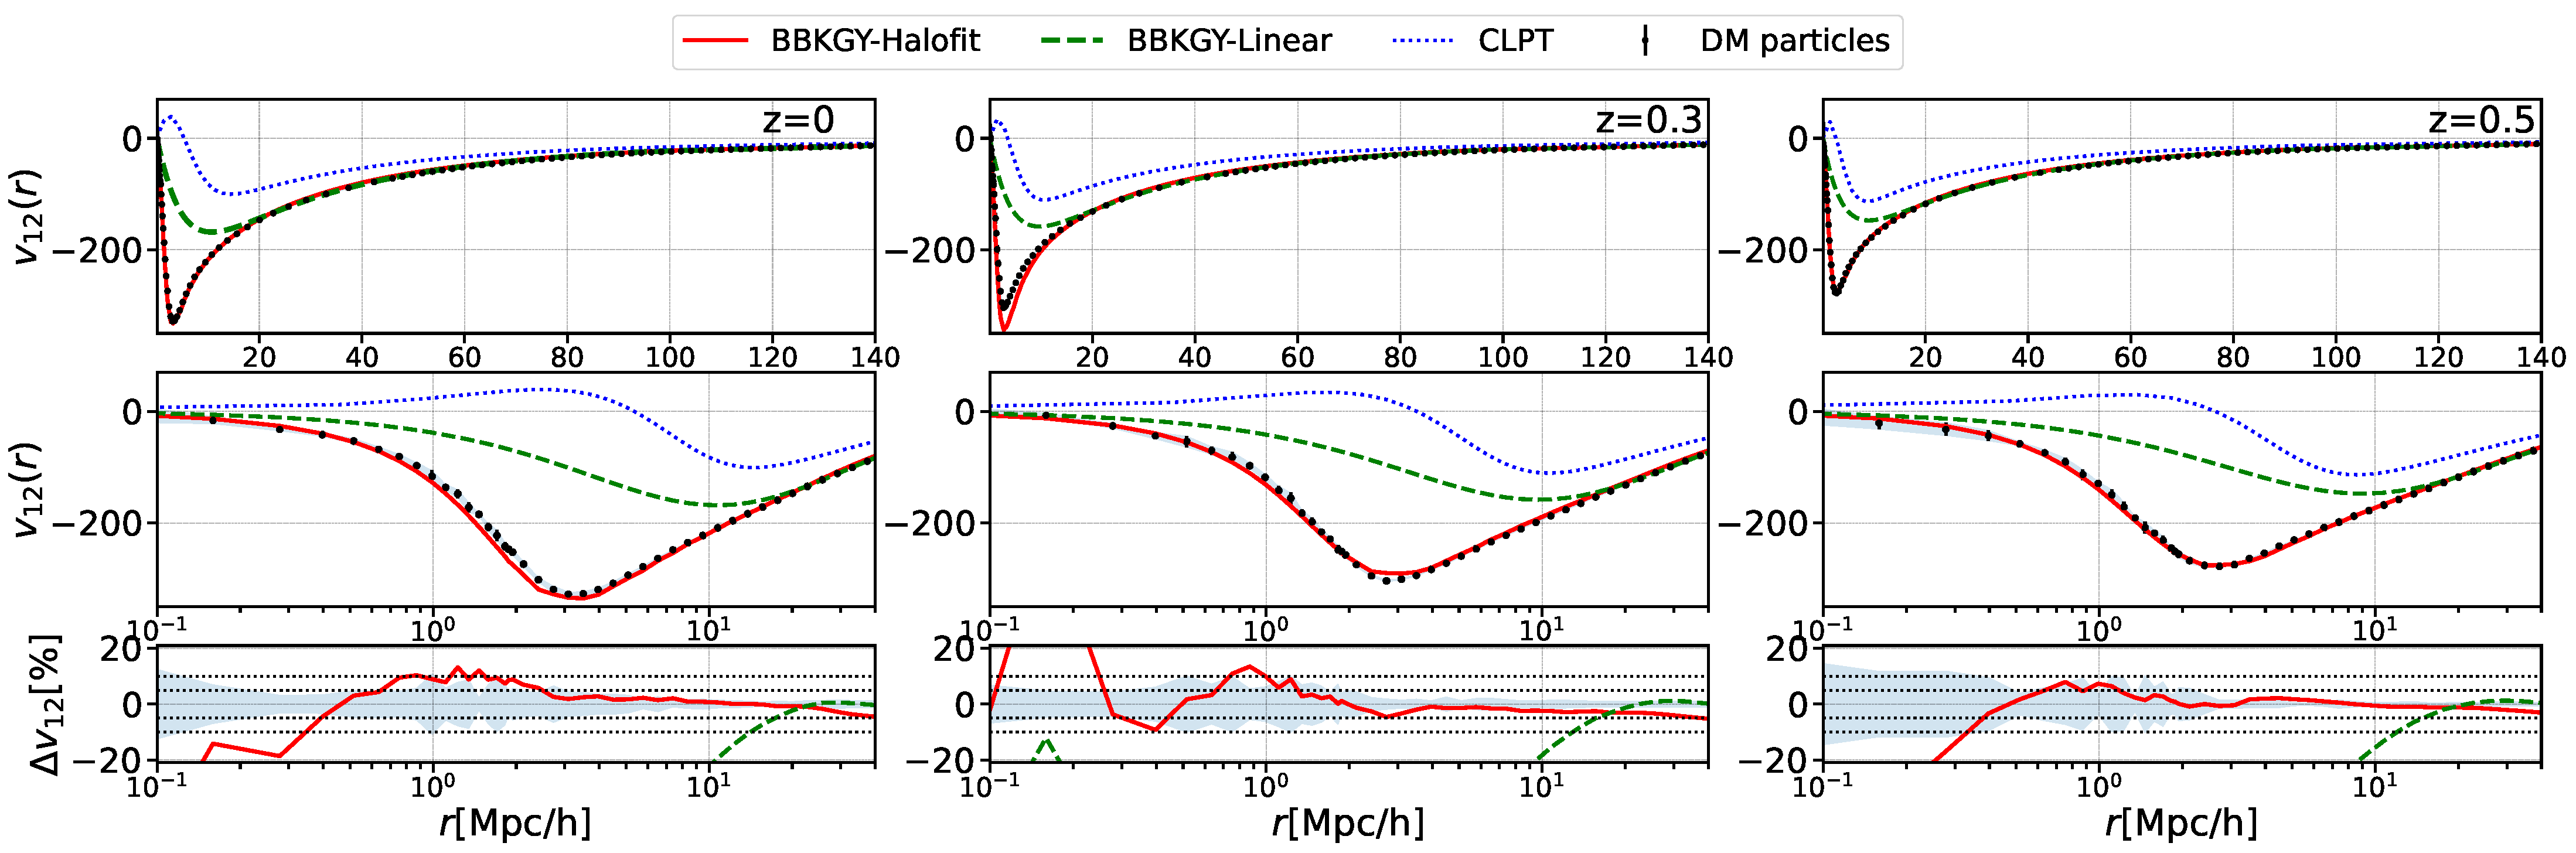
\includegraphics[width=\textwidth]{figs/fig1_v2.pdf}
\caption{\label{fig:v12_model_comparison} Pairwise velocities models for DM tracers. Points correspond to velocities from \elephant{} runs, lines correspond to the different theoretical models: the full solution to \refeq{v12full} using  the linear \code{CAMB} matter power spectrum (dashed green), solution obtained via non-linear \code{halofit} based power spectrum  (solid red), \MJ{(missing): the quasilinear approximation given by eq. \refeq{v12lin} (dot-dashed purple)}, and the prediction from CLPT (dotted blue).}
\end{figure*}
%%%%%%%%%%%%%%%%%%%%%%%%%%
 

%%%%%%%%%%%%%%%%%%%%%%%%%%%%%%%%%%%%%%%%%%%%%%%%%%%%
%%    						METHODS										%%
%%%%%%%%%%%%%%%%%%%%%%%%%%%%%%%%%%%%%%%%%%%%%%%%%%%%
\section{\label{sec:methods}Methods}

We proceed to describe the analytical models, numerical techniques and simulation data we used. The model itself has no explicit cosmology dependence, however its ingredients can be derived either in \lcdm{} or extensions to the standard paradigm.

As we focus on the type of extensions to \lcdm{} called modified gravity (MG) theories, we will outline their main phenomenological consequences, relevant for our results. 
In general,  different prescriptions of the theory of gravity will require a way  of evading the high-density constraints and still allow deviating from GR on cosmological scales. This can be achieved  by what it is called ``screening mechanisms", which are theoretical concepts proposed to reconcile the predictions of GR with experimental observations on cosmological and astrophysical scales, effectively  hiding the modifications to Einstein field equations in these environments. 

The specific theories we consider are \textbf{(1)} the normal branch of the Dvali-Gabadadze-Porrati (nDGP) model which attempts to explain the accelerated expansion of the universe by introducing extra dimensions that affect gravity on large scales while recovering standard GR at small scales \cite{ndgp_2000} and \textbf{(2)} the Hu-Sawicki form of $f(R)$-gravity \cite{HS_fR_2007}, a popular extension of the Hilbert-Einstein action that introduces an universal modified gravity force in a scale-dependent way.  

The first family is an example of  the Vainshtein screening mechanism (VSM) \cite{Vainshtein_1972}, while the particular form of $f(R)$ that we consider implements the Chameleon screening mechanism (CSM) \cite{Khoury2003PRD}. In a nutshell: the Vainshtein mechanism relies on the nonlinearity of the equations of motion for the scalar field, leading to a suppression of its effects at small scales. The Chameleon mechanism, on the other hand, involves a scalar field with a variable effective mass that depends on the local matter density, allowing it to be screened in high-density environments while remaining active in low-density regions.

Now we describe the main core of our model, its ingredients within standard \lcdm{} cosmologies, and in the above mentioned MG theories, as well as the data against which we test our predictions.

\subsection{\label{subsec:model}Model}
Our model relies in the consistent numerical solution of the following equation \cite{Juszkiewicz_1999}:

\begin{equation}
    \label{eq:v12full}
    \frac{a}{3[1+\xi(x,a)]}\frac{\partial\bar{\xi}(x,a)}{\partial a} = - \frac{v_{12}(x,a)}{H(a)r}
\end{equation}
%
where $\bar{\xi}(r,a) = 3x^{-3}\int^x_0\xi(y,a)y^2dy$ and  $r=ax$ is the proper separation.

Before describing the different proposals for the non-linear regime, let us briefly examine the limiting values of \refeq{v12full}. In the case of  pairs separated at $x<<1$ or, equivalently, high values of $\xi >>1$ we recover the \emph{stable clustering} regime. 
%
The opposite case, \emph{i.e.} at large $x$ where $\xi(x,t)\gg1$, we are in what is known as the \emph{linear-regime}.  
Here the growing mode of structure formation dominates and we have $\xi(r, t)=D(t)^{2} \xi(r,t=0)=D(t)^{2} \xi_{0}(r)$. Substituting this result in the pair-conservation equation and solving for
\vot{}, we get:
\begin{equation}\label{eq:v12lin}
v_{12}(x,a)=-\frac{2}{3}axHf\bar{\bar{\xi}}(x,a),
\end{equation}
%
where $\bar{\bar{\xi}}(x,a)\equiv \bar{\xi}(x,a)/[1+\xi(x,a)]$ and $f$ is the logarithmic derivative of the growth function, $f\equiv d\ln D/d\ln a$. 

The turn-over scale between the MPVs being dominated by the Hubble flow versus the stable clustering regime is an important feature that we discuss further in following sections, in particular in the context of different gravity theories. 

\subsection{\label{subsec:pk}Non-linear Power spectrum}

As we aim to model the MPV for sub-Mpc separations, we need to have a model for the non-linear clustering in \refeq{v12full}. To this end we take different proposals for the non-linear power spectrum, $P_{nl}(k,z)$, and Fourier transform them to provide the corresponding non-linear 2PCF, $\xi_{\text{nl}}(r,a)$, needed in \refeq{v12full}.  
 
\textbf{Non-linear clustering in \lcdm{}.} The first model for $P_{nl}(k,z)$ that we use is the \code{Halofit} solution \cite{2019MNRAS.486.1448S, 2012ApJ...761..152T,2015MNRAS.454.1958M} on top of the standard linear matter power spectrum from the cosmological Boltzmann solver \code{CAMB} \cite{Lewis_2000,Howlett_2012}. 
%
This fitting formula is an optimized variant of the known Halo Model (HM), which we use for the \lcdm\-\ case as its accuracy is tested to be up to $\sim5\%$ for $k\leq10$\Mpch{}, and $z\leq2$, for a variety of \lcdm\-\ and wCDM cosmologies. Another alternative is the \code{Euclid Emulator 2 } \cite{2021MNRAS.505.2840E} to obtain the non-linear corrections to the matter linear spectrum. % \MJ{Mention alternatives such as EUCLID EMULATOR?}

Additionally, we also compare it against the results from the Convolution Lagrangian Perturbation Theory (CLPT) \cite{2013MNRAS.429.1674C}, which is a    non-perturbative resummation of Lagrangian perturbation theory and provides as an output, an estimation for \pairvel{}.   



\textbf{Non-linear clustering in MG.}
%
For models that deviate from the standard paradigm such as the Modified Gravity scenarios we consider, there is less consensus regarding how to optimally model the non-linear power spectrum. Some proposals compute it  either directly on N-body simulations \citep{PhysRevD.78.123524, Alam_2021}, using perturbation theory \citep{PhysRevD.79.123512},  post-Friedman formalism (PPF)  \citep{PhysRevD.76.104043}, or by means of the spherical collapse model \citep{10.1093/mnras/stv2036}. A MG-Halofit has been proposed in \citep{Zhao_2014} specifically for $f(R)$. Nonetheless, it is important to acknowledge that these works rely on several underlying assumptions, and possess certain limitations, thereby restricting their applicability and generality.

Instead, we rely on the recent proposal of \cite{2023PhRvD.107h3525G} to compute the MG non-linear matter power spectrum.  This approach requires two primary inputs: {\textbf{(i)}} The halo model (HM) construction for both MG and \lcdm{}, and {\textbf{(ii)}} a user-specified input to compute the non-linear power spectrum for \lcdm{}. The accuracy of this method will be provided by the performance of the input \lcdm{} predictions


The resulting non-linear matter power spectrum for MG, $P(k)_{\text{nl, MG}}(k)$, can be expressed in terms of the input non-liner power spectrum for \lcdm{},  $P(k)_{\text{nl}, \Lambda \text{CDM}}(k)$, and a response function, $\Upsilon(k)$:
\begin{equation}
\label{eq:pkmg}
    P(k)_{\text{nl, MG}}(k) = \Upsilon(k) \times P(k)_{\text{nl}, \Lambda \text{CDM}}(k).
\end{equation}
%
There, $P(k)_{\Lambda \text{CDM}}$ is the non-linear \lcdm\ power spectrum and can be specified by the user. 
For our analysis, we utilize the \code{halofit} predictions for $P(k)_{\Lambda CDM}$, employing the parameters corresponding to the given background cosmology, as we have used the same for the \lcdm{} case.

The power of this proposal lies in their response function, $\Upsilon(k)$, which is the ratio of the halo model predictions of MG to \lcdm{} power spectrum, i.e.,  $\Upsilon(k) = P(k)_{\text{MG, HM}}/P(k)_{\Lambda\text{CDM, HM}}$. The precise ingredients of the HM for MG were discussed in  \cite{2023PhRvD.107h3525G}. 

While the work of   \cite{2023PhRvD.107h3525G}  specifically focuses on $f(R)$ and nDGP modified gravity models, their  approach can be readily extended to other modified structure formation models.

The resulting power spectrum for the MG models considered reaches a 5\% accuracy up to non-linear scales of $k \lesssim 2.5-3$\Mpch. 

We then compare our prediction using those different solutions against the direct estimation for \pairvel{}  from a full N-body simulation. 
Below we describe the data we have used. 

%%%%%%%%%%%%%          figure 2           %%%%%%%%%%%%% 
\begin{figure*}
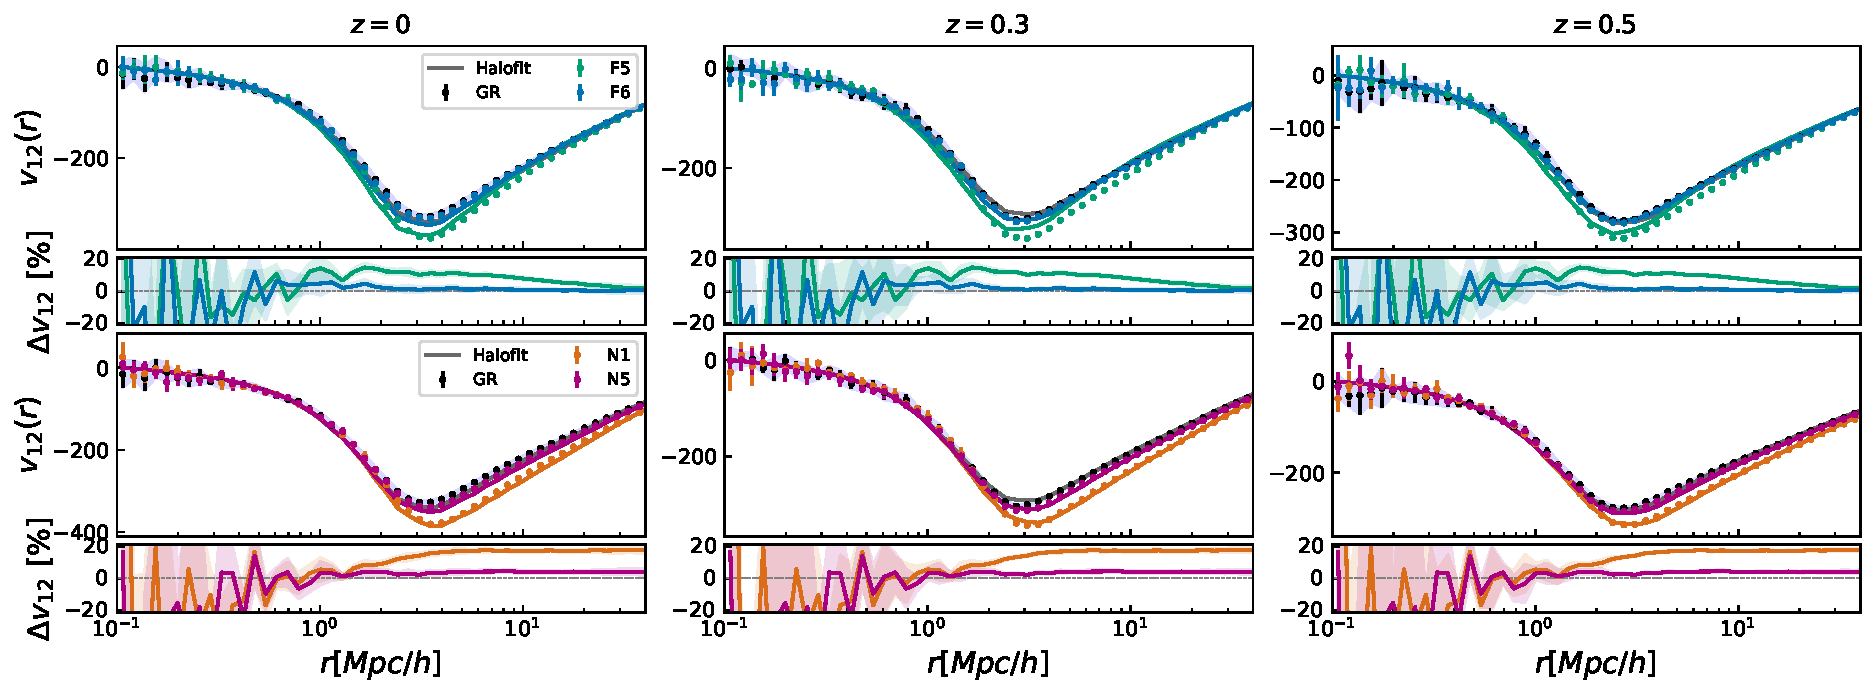
\includegraphics[width=\textwidth]{figs/fig2_v12datamodelMG_all.pdf}
\caption{\label{fig:v12_model_comparisonMG} Pairwise velocities models for DM tracers in MG models. Points correspond to DM particles from \elephant runs, lines correspond to the \code{halofit} prediction. \MJ{WORKING ON THIS figure} }
\end{figure*}
%%%%%%%%%%%%%%%%%%%%%%%%%%%%%%%%%%%%%%%

%%%%%%%%%%%%%          figure 3           %%%%%%%%%%%%% 
\begin{figure*}
    \centering
    \begin{subfigure}[c]{0.45\textwidth}
        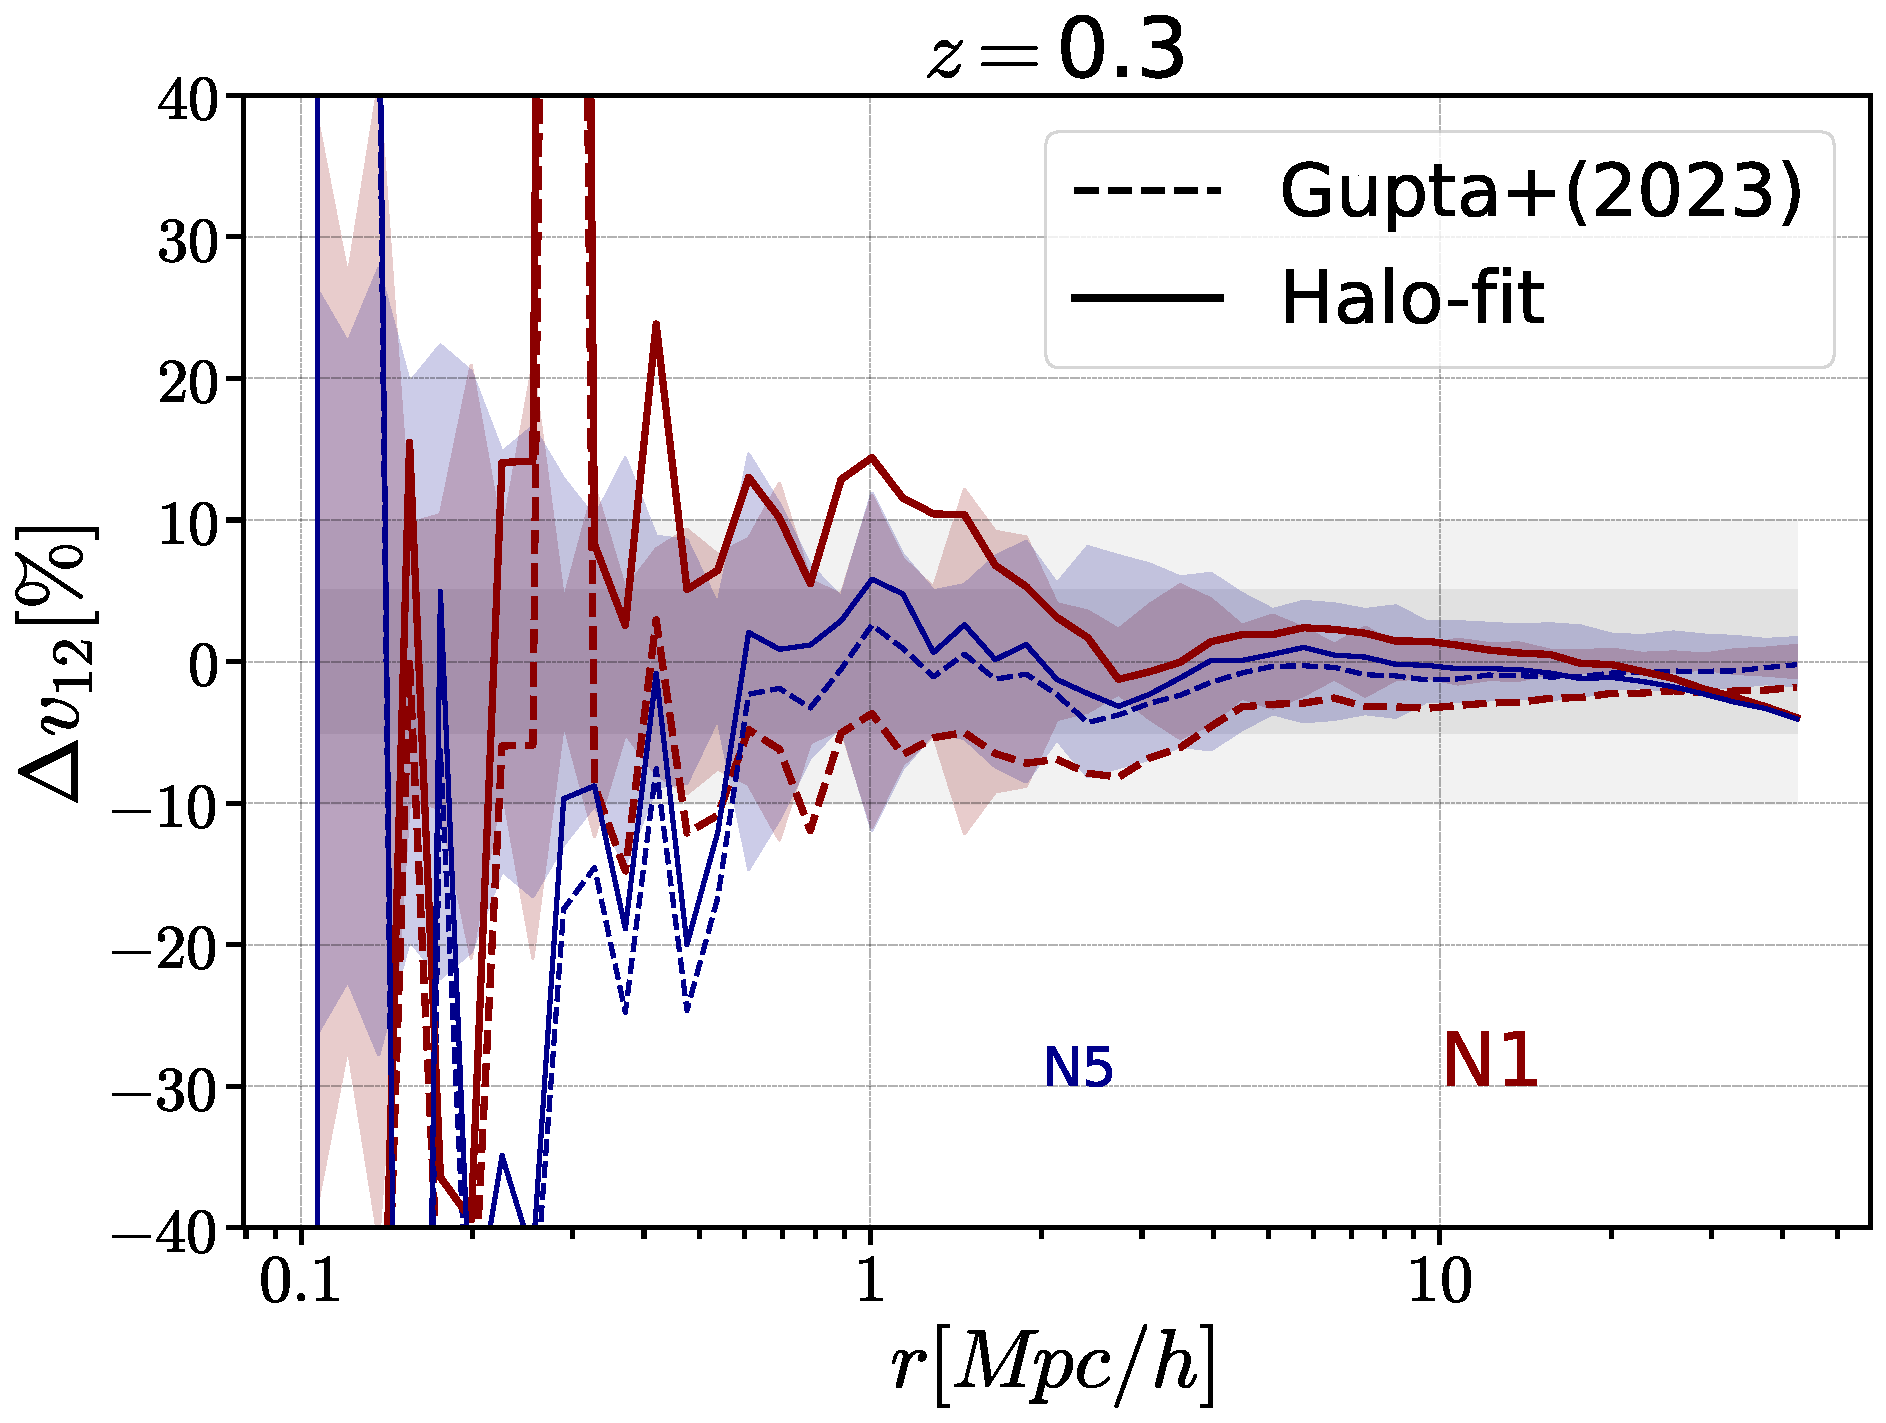
\includegraphics[width=\textwidth]{figs/shaded_ratio_v12_HM_HF_N1_N5z03}
        \label{fig:ndgp}
    \end{subfigure}
    %
    \begin{subfigure}[c]{0.45\textwidth}
        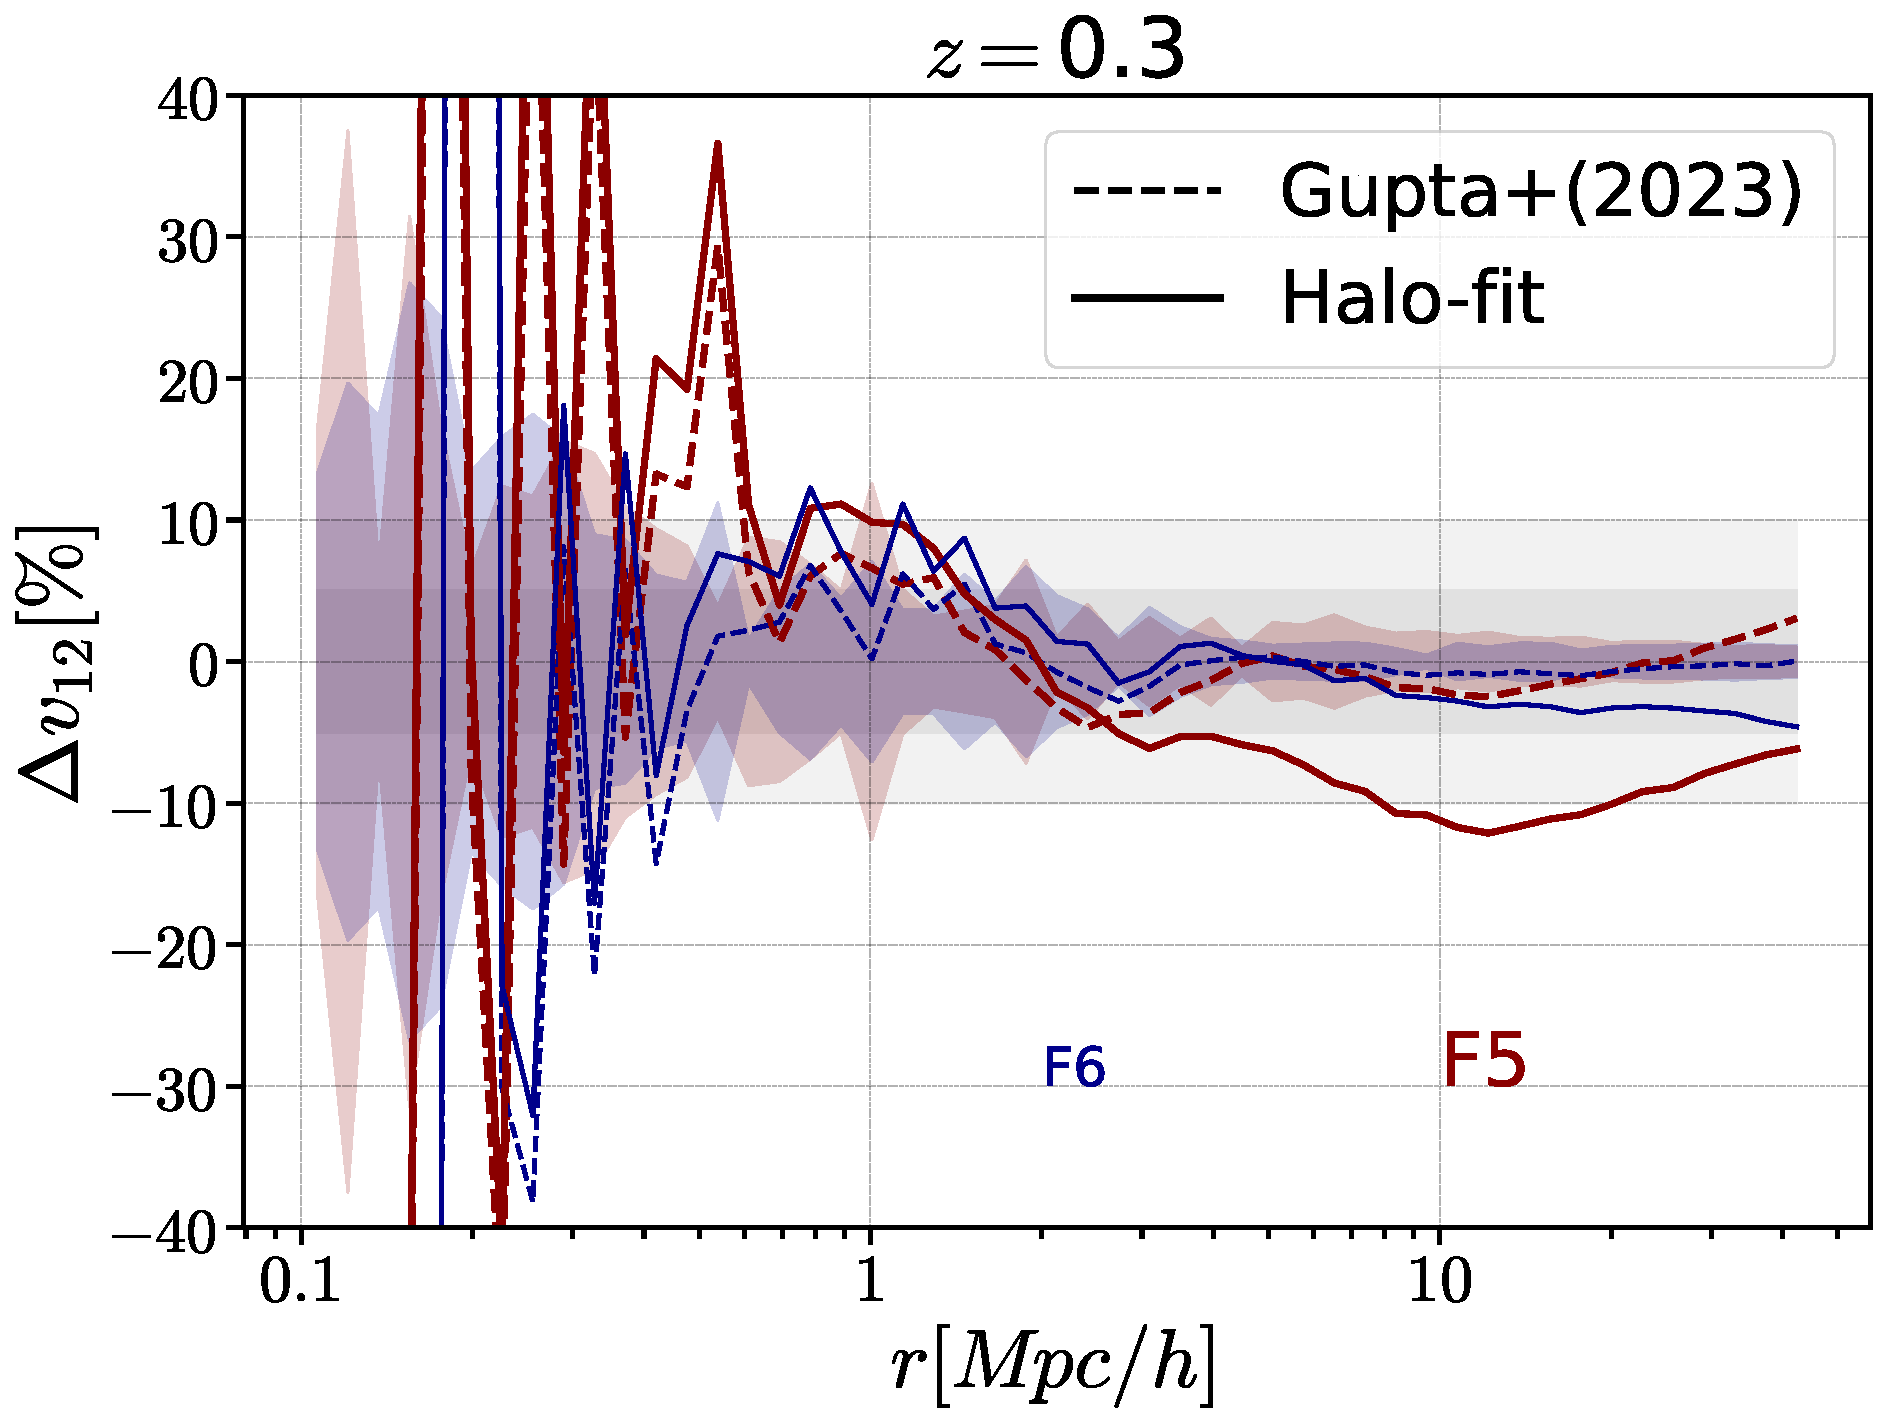
\includegraphics[width=\textwidth]{figs/shaded_ratio_v12_HM_HF_F5_F6z03}
        \label{fig:fofr}
    \end{subfigure}
    \caption{Halo model for MG.  \WH{is this a dummy(place-holder) caption or you intend to keep it so generic? I think some more text and description would be good here.}}\label{fig:hm}
\end{figure*}
%%%%%%%%%%%%%%%%%%%%%%%%%%%%%%%%%%%%%%%


%%%%%%%%%%%%%%%%%%%%%%%%%%%%%%%%%%%%%%%%%%%%%%%%%%%%
%%    			DATA										%%
%%%%%%%%%%%%%%%%%%%%%%%%%%%%%%%%%%%%%%%%%%%%%%%%%%%%
\subsection{\label{subsec:data}Data}

We use data generated from the suite of DM-only MG $N$-body simulations: \elephant{}(Extended LEnsing PHysics using ANalytic ray Tracing), \citep{ALAM2020_ELEPHANT}, as these simulations provide a good test-bed to study the impact of the Chameleon and Vainshtein screening mechanisms on the large scale non-linear clustering of matter  described above.

This set of  $N$-body simulations assumes a \lcdm{} background, and implements on top of this the solution of the scalar field and modified Einstein equations in the MG models: normal branch of the DGP theory, or nDGP, and  the Hu-Sawicki form of $f(R)$. In the first case, the specific values of the extra parameter are: $Hr_c = 1, 5$ (referred to as  N1 and N5, respectively), and for the second model, the strenght of the modification is codified by the present-day value of the derivative of the function $f(R)$, $\log(f_{R0})$, taking the values $10^{-5}$, and $10^{-6}$ (refered to as F5 and F6, respectively).  In a similar way, N1 codifies a model that deviates more strongly from GR than N5, just as F5 deviates more from GR than F6. 

%Generally speaking, we can say that F5 has a stronger deviation from GR than F6, and N1, %In this way, we have for F5 a stronger deviation from GR than F6, and N1, a stronger deviation from GR than N5). 


 %with the specific values of the extra parameter, $Hr_c = 1, 5$, referred to as  N1 and N5, respectively, and  the Hu-Sawicki form of $f(R)$ with the present-day value of the derivative of the function $f(R)$, $\log(f_{R0})$, taking the values $10^{-5}$, and $10^{-6}$, refered to as: F5 and F6 (with F5 a stronger deviation from GR than F6, and N1, a stronger deviation from GR than N5). 

These simulations were run using the \textsc{ecosmog} code \cite{ECOSMOG_1,ECOSMOG_V_1,ECOSMOG_2}, for 1024$^{3}$ particles, in a box of size 1024 h/Mpc, from $z_\mathrm{in}=49$, down to $z_\mathrm{f}=0$. 
The mass resolution is $m_p=7.798\times10^{10}M_{\odot}h^{-1}$, and comoving force resolution of $\varepsilon=15$\kpch. 
For each model and each redshift, we have five independent realisations. 
Each MG model has the same fiducial background, with cosmological parameters: $\Omega_m=0.281$ (total fractional non-relativistic matter density), $\Omega_b = 0.046$ (fractional baryonic matter density),
$\Omega_\nu = 0.0$ (fractional relativistic matter species density), $\Omega_{\Lambda}=0.719$ (cosmological constant energy density), $\Omega_k=0$ (fractional curvature energy density), $h=0.697$ (Hubble constant in units of 100 \kps\,Mpc$^{-1}$), $n_s = 0.971$ (primordial power spectrum slope), and $\sigma_8 = 0.842$ (linearly extrapolated \lcdm{} power spectrum normalization). 

For the direct counting in the simulation data, we use the positions and velocities of a $1\%$  subsample of the dark-matter particles and analyse the snapshots at $z = 0, 0.3$ and $0.5$. %randomly chosen


%%%%%%%%%%%%%%%%%%%%%%%%%%%%%%%%%%%%%%%%%%%%%%%%%%%%
%%    	RESULTS								%%
%%%%%%%%%%%%%%%%%%%%%%%%%%%%%%%%%%%%%%%%%%%%%%%%%%%%

%%%%%%%%%%%%%%		figure 4  		%%%%%%%%%%%%%%%%%

\begin{figure*}
    \centering
    \begin{subfigure}[c]{0.45\textwidth}
         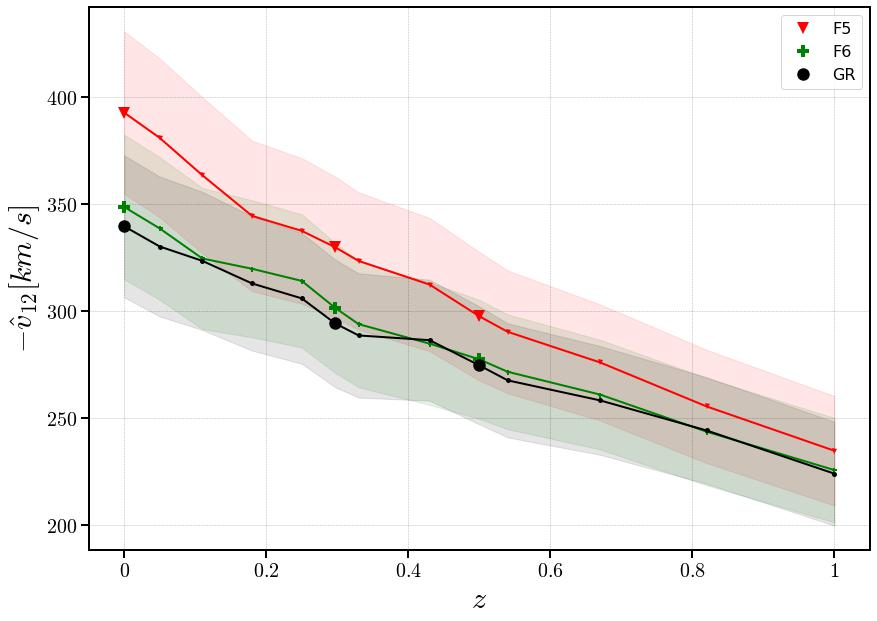
\includegraphics[width=\textwidth]{figs/Peak_v12_FofR_all_zs_cut_err.jpg}
         \caption{Maximum pairwise velocity/turnover peak $\hat{v}_{12}(z)$ as function of redshift for $f(R)$-gravity.}\label{fig:peakv12_fofr}
     \end{subfigure}
    % 
     \begin{subfigure}[c]{0.45\textwidth}
         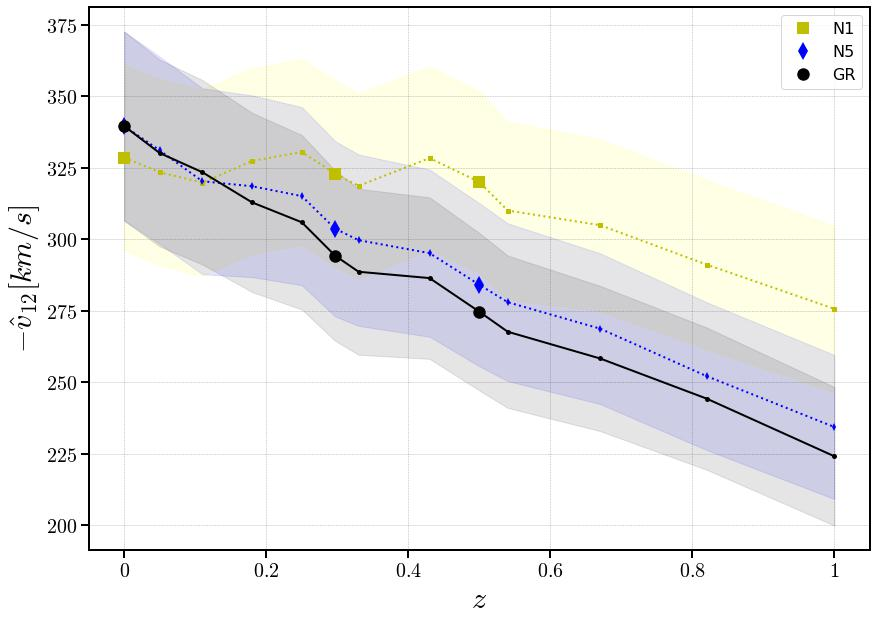
\includegraphics[width=\textwidth]{figs/Peak_v12_nDFP_all_zs_cut_err.jpg}
         \caption{Maximum pairwise velocity/turnover peak $\hat{v}_{12}(z)$ as function of redshift for nDGP-gravity. }\label{fig:peakv12_ndgp}
     \end{subfigure}
    \caption{Maximum pairwise velocity/turnover peak $\hat{v}_{12}(z)$ as function of redshift for all the models. Errors are estimated as averages over 4 bins }\label{fig:peakv12}
\end{figure*}
% \begin{figure}
%     \centering
%     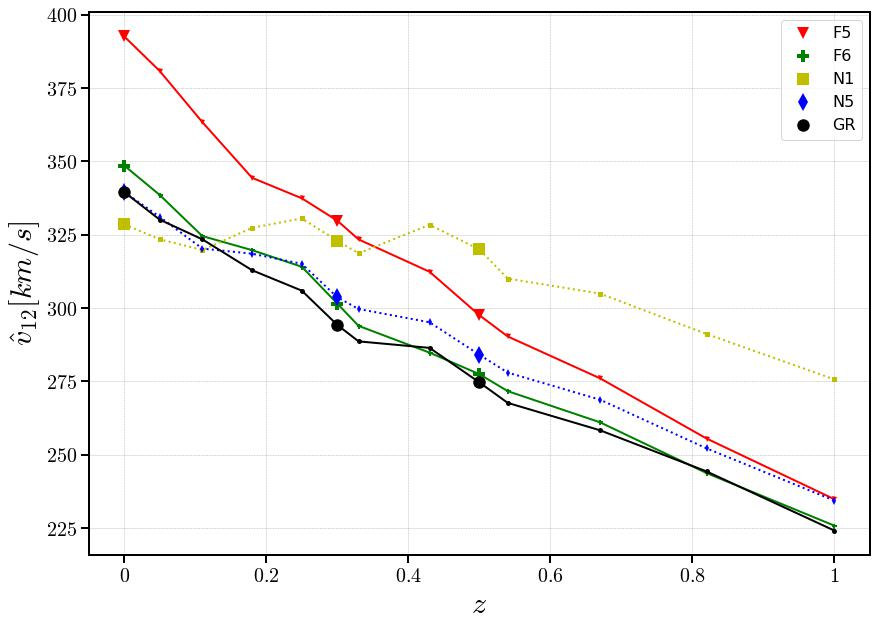
\includegraphics[width=0.5\textwidth]{figs/Peak_v12_all_models_all_zs_cut}
%     \caption{Maximum pairwise velocity/turnover peak $\hat{v}_{12}(z)$ as function of redshift for all the models.  \MJ{ADD ERRORS. FIX Y-AXIS: Minus sign in y-axis label }}
%       \label{fig:peakv12}
% \end{figure}
%%%%%%%%%%%%%%%%%%%%%%%%%%%%%%%%%%%%%%%


%%%%%%%%%%%%% 	figure 5		%%%%%%%%%%%%%%%%%
\begin{figure*}
    \centering
    \begin{subfigure}[c]{0.45\textwidth}
         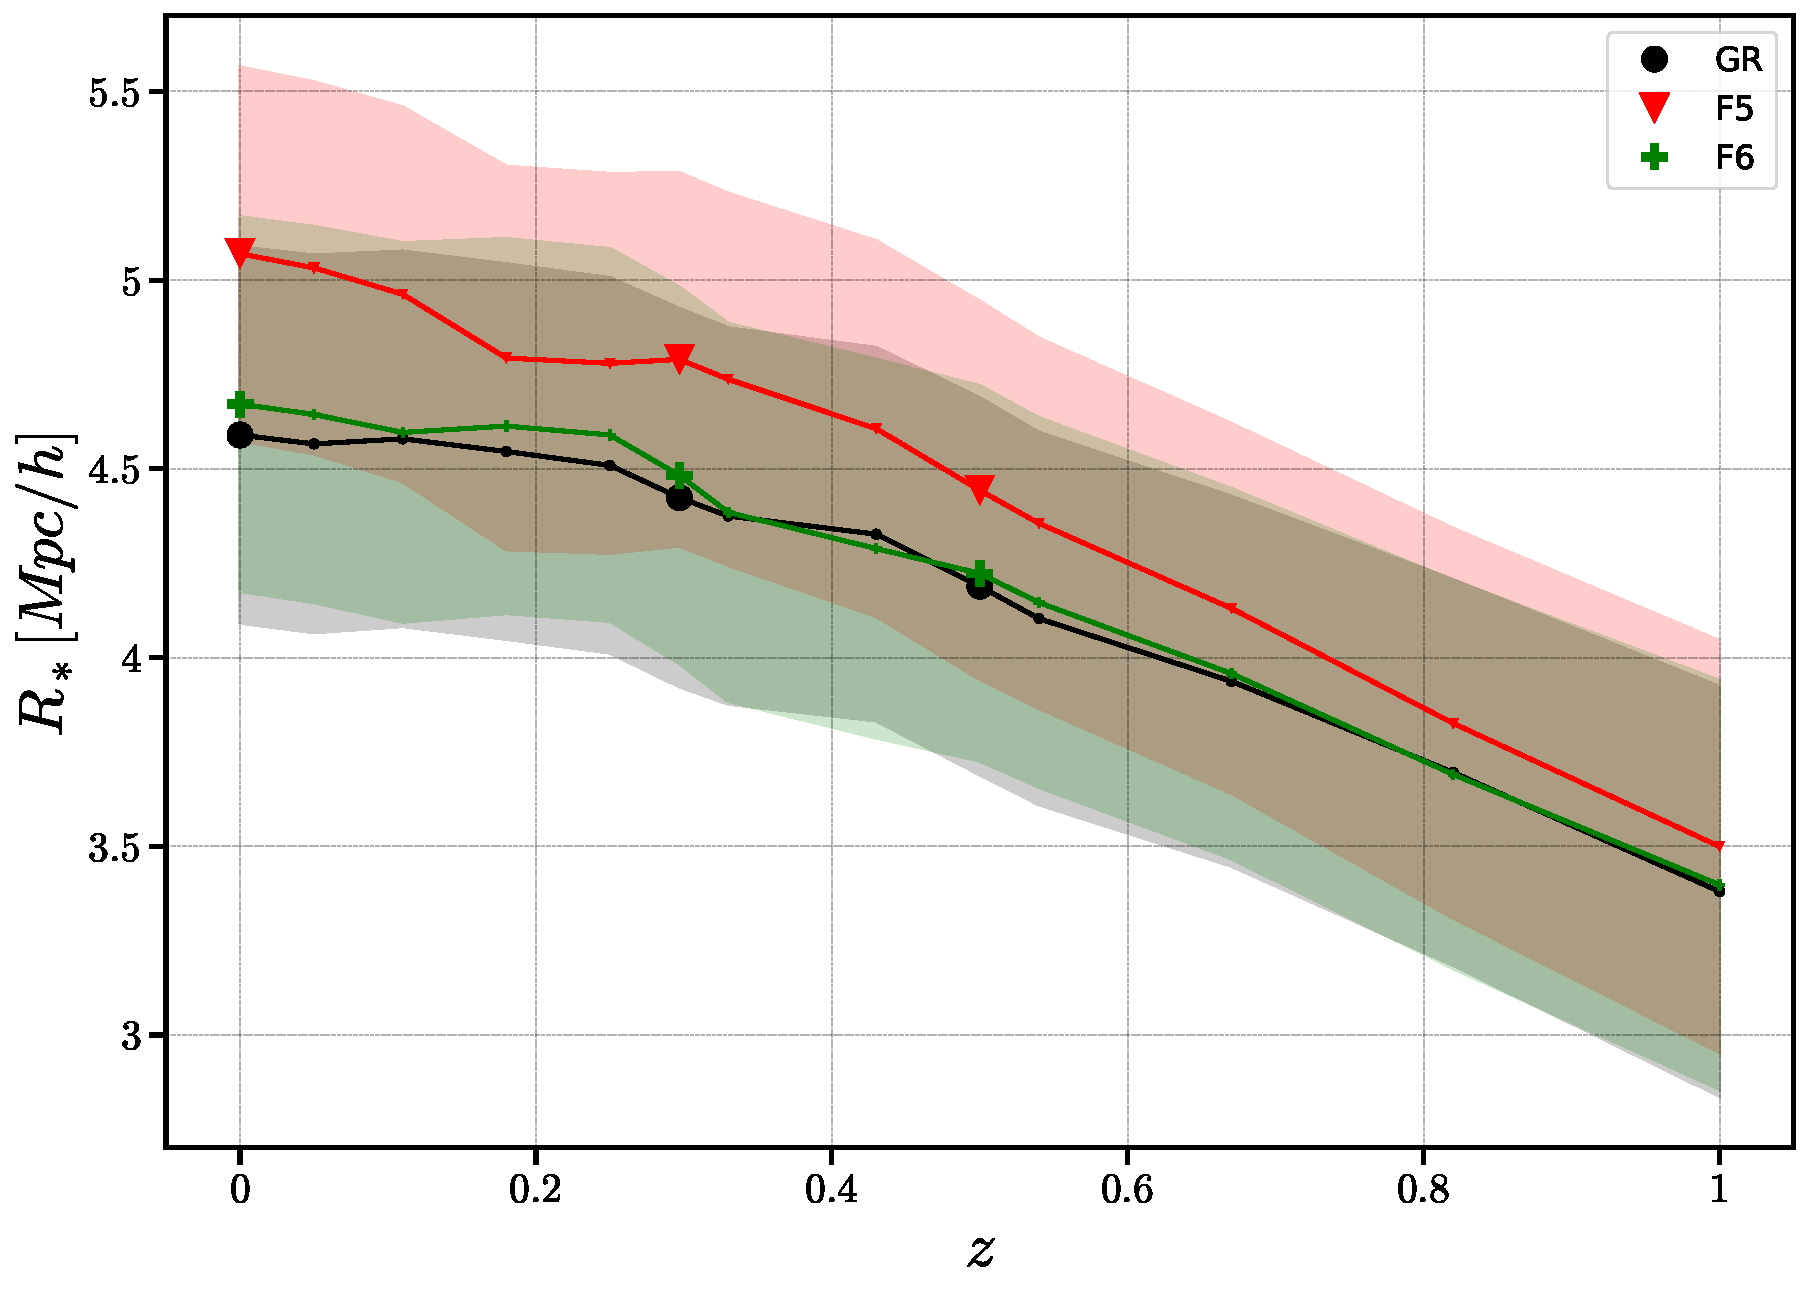
\includegraphics[width=\textwidth]{figs/StableClustering-z_cut_minor_fixed_fofr_err.pdf}
         \caption{Crossing of the stable clustering regime for $f(R)$-gravity.}\label{fig:rstar_fofr}
     \end{subfigure}
    % 
     \begin{subfigure}[c]{0.45\textwidth}
         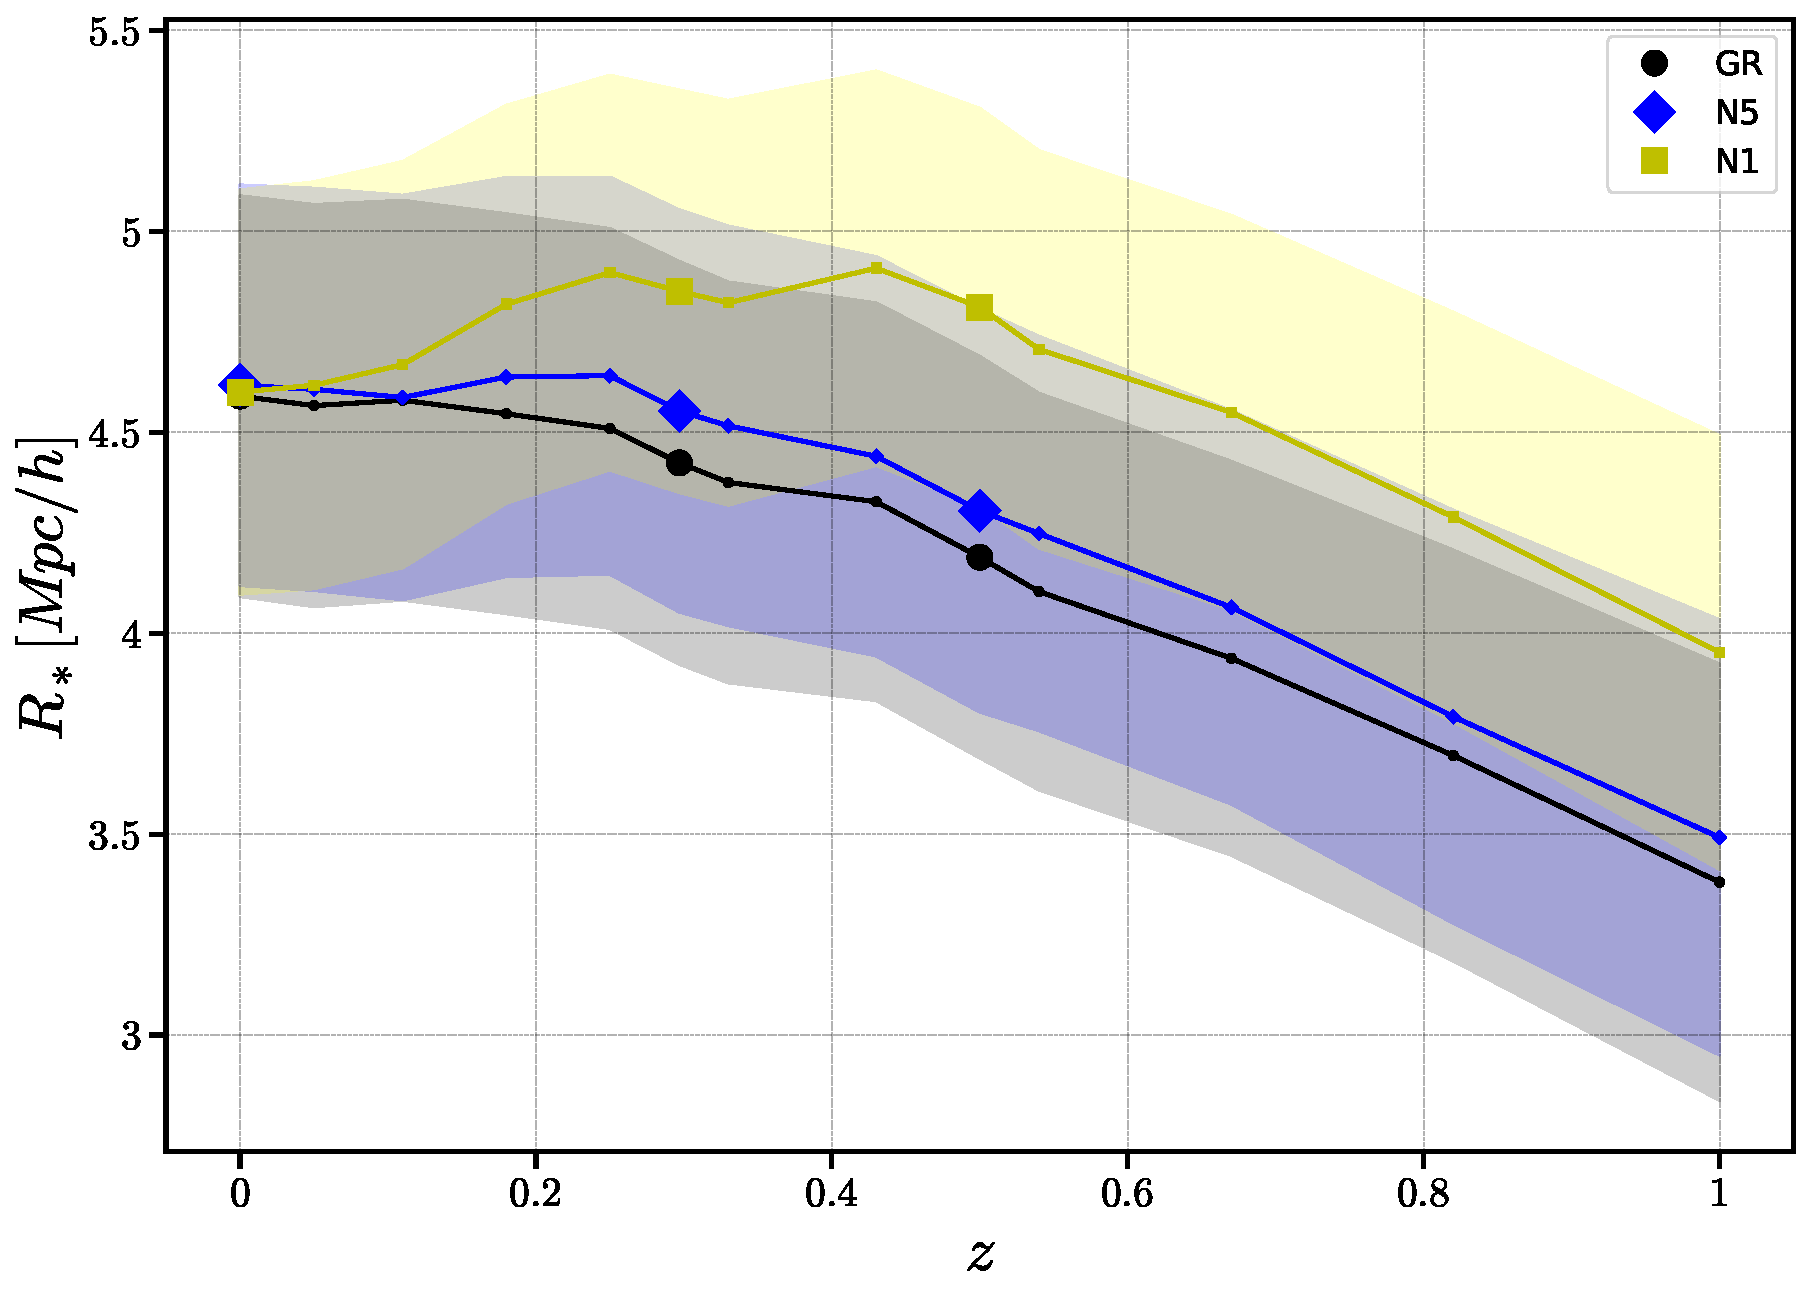
\includegraphics[width=\textwidth]{figs/StableClustering-z_cut_minor_fixed_ndgp_err.pdf}
         \caption{Crossing of the stable clustering regime for the nDGP models}\label{fig:rstar_ndgp}
     \end{subfigure}
    \caption{Scale of crossing the stable clustering regime. Errors are estimated as averages over 4 bins.}\label{fig:rstar}
\end{figure*}
%%%%%%%%%%%%%%%%%%%%%%%%%%%%%%%%%%%%%%%


\section{\label{sec:results}Results}

We present our results related to the modeling of MPVs in the non-linear regime. We begin by presenting the case of \lcdm\-\ and discuss our model in the context of other solutions. Then we move to analyzing the applicability of our model for Modified Gravity schemes.

\subsection{\label{subsec:resultslcdm} Mean Pairwise Velocities}
\textbf{MPV for the \lcdm{} model.}
The resulting solution for \refeq{v12full} is shown in the different panels of \reffig{v12_model_comparison}.  From left to right we show the solution at different redshift values. The top row includes our solution for values of $r \in 0.01-140$\Mpch, in order to cover the linear and non-linear regimes simultaneously. The middle row zooms in the region $r \in 0.01-40$\Mpch, to emphasize the behaviour of our solution in the non-linear regime. The bottom row panels present the ratio of our numerical solution for \pairvel{} with respect to the simulation data, $\Delta$\vot{}$\equiv (v_{12, \text{sim}}-v_{12})/v_{12, \text{sim}}$. The direct count from the simulation N-body particles, or $v_{12, \text{sim}}(r)$, is indicated by black dots and the error bars represent the variance of the five independent realisations of each snapshot.

Additionally to the solution for \refeq{v12full}  with the \code{halofit} prescription (``BBKGY-Halofit"), we also solve it using the linear power spectrum directly output by \code{CAMB}. This is indicated by green dashed lines, labeled as ``BBKGY-linear".

For comparison with the results of \cite{Juszkiewicz_1999}, we also include the solution to \refeq{v12lin}  using the \code{halofit} non-linear power spectrum as input. This is represented by purple dot-dashed lines and labeled as  ``quasi-linear"  solution. 

The last  model included in \reffig{v12_model_comparison} is the solution for \pairvel{} from the numerical implementation of \code{CLPT}\footnote{\href{https://github.com/wll745881210/CLPT_GSRSD}{https://github.com/wll745881210/CLPT-GSRSD}}, which provides as output the real-space pairwise in-fall velocity in units of $v/aH(a)f$. This is shown in \reffig{v12_model_comparison} as  dotted blue lines. 

The first thing to notice is the agreement of all the solutions on scales $r\geq 80$\Mpch. This is to be expected as those scales are well inside the linear-regime, where the Hubble expansion drives the dynamics of pairwise velocities. 
%
The results from CLPT were optimised for galaxy  clustering analysis, in particular to extract the baryonic acoustic oscillations (BAO) feature from the 2PCF of biased tracers, therefore, it provides a good solution around BAO scales ($r_{BAO} \sim 100$ \Mpch).
%
However, we notice that for separations below  $r \sim 80$\Mpch, this perturbative solution and the ``quasilinear" solution  %(\refeq{v12lin} with $\xi_{\text{Halofit}}(r,a)$) 
both  start to deviate with respect to the simulation data and the other solutions. 
This is better shown in the middle row panel, where we focus on separations below  $r= 40$\MpchInv{}: the CLPT solution follows the behaviour of the quasilinear solution up to $r\sim11$\MpchInv{} and then departs the most at the non-linear regime. The ``BBKGY-linear" solution  performs better than the previous two cases: it follows the evolution of the simulation data within 5$\%$ of accuracy up to separations of $r\sim11$\MpchInv{} (across all redshift values), then, it deviates in the intermediate and non-linear regimes. 

Lastly, the fully non-linear solution of \refeq{v12full} with $P_{\text{non-lin}}(k)$ from \code{halofit} follows the dynamics of the direct count of pairs of DM particles in the simulation with an accuracy of $\sim 5\%$ (\MJ{quote the 10 percent instead?}) up to separation of $r\sim0.6, 1.2, 1$\MpchInv{}, for $z=0, 0.3, 0.5$, respectively. 

The time evolution of our solutions across the snapshot values $z=0, 0.3, 0.5$, shows similar behaviour with respect to the simulation data with decreasing overall value of \pairvel{} in the lowest point for earlier snapshots. This feature will be analyzed in detail in the context of different gravity models.\MJ{check the plot!!! }

\textbf{MPV in MG theories.}

For the models extending \lcdm{} as in the MG theories we consider, we first discuss the outcome from \refeq{pkmg} setting the response function to  $\Upsilon(k) =1$. %, or using the calibration derived by \cite{2023PhRvD.107h3525G}. 
The results from this can be seen in \reffig{v12_model_comparisonMG}, where we have three columns, showing the three snapshots from the simulations: from left to right, $z=0, 0.3, 0.5$. 

For clarity we divided the results from this figure in two rows: the top row has the results for $f(R)$-gravity, while the bottom row has the results for the nDGP case.  For each case we plot the evolution of \pairvel{} in the range $r\in[0.1, 40]$\Mpch{} from the solution of \refeq{v12full}  together with the direct pair counting in the simulation data: in black for the GR simulation box, and color coded, for the corresponding MG model. The errors (shaded region) were estimated as the variance of the 5 independent realisations for each snapshot. In each case we include a subplot showing the ratio of the solution for \pairvel{} w.r.t. the corresponding MG model simulation: $\Delta$\vot{}$\equiv (v_{12, \text{sim}}-v_{12})/v_{12, \text{sim}}$. 

Reading \reffig{v12_model_comparisonMG} from left to right, we see that the time evolution is captured by our model, even in this non-\lcdm{} scenarios.

For the Hu-Sawicki $f(R)$ model with F5 (green dots) and F6 (blue dots), we can see that the simulation results from the F6 case follow closely the evolution from the GR case, but there is a difference in the amplitude of the dip between the GR data and the F5 data. This trend is captured by the corresponding model for \pairvel{} (shown in solid blue and green lines, respectively). To better appreciate how the dynamics of pairwise velocities are captured by our model within the $f(R)$ framework we refer to the ratios $\Delta v_{12}$ shown in the subplots. Generally speaking we can see that the accuracy with which our model for \pairvel{} captures the dynamics from the MG simulations is better than $10\%$ \MJ{this numbers will change with new errors} for pairs separated at scales  $r \geq 10$\MpchInv{}.  For a weaker modification of GR (as in F6), the discrepancy between our model and the data is smaller than $5\%$ for the same range in $r$.

It is worth pointing out that the solution for \pairvel{} plotted in \reffig{v12_model_comparisonMG} comes from the \code{halofit} correction on top of the linear matter power spectrum of the Boltzmann solver for MG, \code{MGCAMB}: a modified version of \code{CAMB} implementing routines to solve both the $f(R)$ and nDGP gravity models.\MJ{references needed}. 
%
As said before, this corresponds to setting $\Upsilon(k)=1$ in \refeq{pkmg}. 

In this $f(R)$-gravity, we notices that as we go to larger scales (separations $r>$ few tens of \Mpch), the modifications w.r.t. GR decrease, effectively recovering the GR prediction and therefore our model for \pairvel{} matches the direct pair-counting in the simulation data.  \MJ{noisy results at small separations: to be fixed in new data. }

Moving on to describe our nDGP results (bottom row of \reffig{v12_model_comparisonMG}), we see an even larger difference (up to $\sim20\%$)  between our prediction and the data, in particular for the stronger deviation from GR, which in this case is represented by the N1 model. The N5 result agrees with the data within $5\%$ for pairs separated  by distances larger than $r\simeq1$\Mpch. Since the Vainshtein mechanism screens the effects at small scales, as we move to larger scales we can appreciate a constant shift between the model for N1 and the simulation data. The same trend, but of smaller magnitude is present for the N5 case, as expected.%The Vainshtein screens at small scales 

%However, to test the non-linear model for MG described in \refeq{pkmg}, with the response functions properly callibrated for the MG models here considered, we show its performance for the four variants: N1, N5, F5, and F6, in \reffig{hm}. 


However, properly accounting for the non-linear clustering in MG by following the prescription for $P_{\text{MG,non-lin}}(k)$ stated in \refeq{pkmg} has a significant impact in the modeling for \pairvel{}. This is demonstrated in our \reffig{hm}, where we show the nDGP results in the left panel, and the HS $f(R)$-gravity in the right panel. 
%
As we already saw that the model correctly captures the time evolution, we show only the results at $z=0.3$.
%
Here we compare the solution using $\Upsilon(k)=1$ (\lcdm{}-Halofit on top of the MG $P_{lin}(k)$), labeled as ``Halofit" (solid lines), and the fully non-linear model (with $\Upsilon(k)$ calibrated as in \cite{2023MNRAS.522.5291G}), labeled as ``Gupta+2023" (dashed lines), against the simulation data. For each panel we represent the stronger modification to GR with thicker lines (N1 or F5), than the ones closer to GR (N5, or F6).

In the case of nDGP (left plot in \reffig{hm}),  we notice a marked improvement in the $\Delta v_{12}$ between the non-linear model from \refeq{pkmg} and the Halofit solution. For the weaker modification of gravity, N5 case, this two solutions are within $5\%$ or better for pairs separated  above $r\sim600$\kpchInv (blue lines). For a stronger deviation from GR, as in N1 (red thick lines), then we see that the ``Gupta+2023" solution is within $5\%$ of the simulation data for scales above $r\sim4$\MpchInv, while the Halofit solution reaches the same accuracy for separations above  $r\sim1-2$\MpchInv. \MJ{re-check the larger separations, in this plot we do not have the 20 percent difference as in the plot above}.

The results for $f(R)$ are similar, in the sense that the weaker modification (or F6, in blue thin lines) follows closely the dynamics of the simulation data for pairs separated at $r \geq2$\MpchInv. For F6, both solutions, the Halofit result (solid line) and the model of ``Gupta+2023" (dashed line)  give similar results, but we notice the increased precision in the latter case, while the Halofit solution deviates within $5\%$ for large separations ($r>20$\MpchInv). For F5, however, the differences between using both solutions are prominent (dashed vs solid thick-red lines). The Halofit solution deviates from the simulation data at all scales within our range, while the solution for \refeq{pkmg} gives a prediction within $5\%$ or better for pairs separated up to $r\sim1$\MpchInv. \MJ{re-check the larger separations, in this plot we do not have the 20 percent difference as in the plot above}.


\subsection{\label{subsec:mgsignatures} Signatures of MG in the MPVs}

Interesting features arise form comparing the pairwise dynamics in different gravity models. As we have already noticed in \reffig{v12_model_comparisonMG}, with stronger deviations from GR we can notice a deeper minimum of \pairvel{}, compared to weaker deviations from GR and GR itself. \MJ{error bars will be added}

To quantify this, in \reffig{peakv12}, we show the value where \pairvel{} reaches its minimum, denoted by  $\hat{v}_{12}$, \MJ{FIX Y-AXIS: add a minus sign in the plot label}, as function of redshift, $z$, for the different models under scrutiny. 

As expected, for earlier times, the relative velocities reach smaller values compared to the present day, so, in all the cases shown in \reffig{peakv12}, we have a tendency towards smaller $\hat{v}_{12}$ (shallower curves for \pairvel{}). The interesting effect is to look at how this value varies across models: for the $f(R)$ case we have a roughly constant shift towards higher values of $\hat{v}_{12}$ for increasing $z$, with respect to GR, pointing out that this gravity model enhances the in-fall pairwise velocities.  Interestingly, the value for F5 increases considerably with respect to GR at $z=0$, showing an \MJ{$X\%$ increase}. At earlier times, however, this values get closer \MJ{quantify relative difference, quote on the context on the uncertainties}. The case of F6 follows very closely the evolution of the peak  $\hat{v}_{12}$ in GR, showing a maximum discrepancy of \MJ{quote $x\%$ } with respect to GR at $z=0$.

For the nDGP gravity we observe a different behaviour. The minimum value of \pairvel{} is roughly the same for N1 and N5 than for GR at present time, or $z=0$, and shows deviations with respect to GR for earlier times. The case of N5 follows closely the time evolution of  $\hat{v}_{12}$ in the GR model, with a maximum departure at $z=1$ of \MJ{$\approx N\%$}.  This departure from GR is intensified in the N1 case, in which case we find similar values for  $\hat{v}_{12}$ at $z=0$, and an increase of this value for $z=1$ of \MJ{$\approx N\%$ 50km/s}. 

%\MJ{MISSING: DESCRIBE crossing into the stable clutering regime \reffig{rstar} }

A separate interesting feature is the scale at which each model crosses into the stable clustering regime. We denote this scale as $R_*$. To solve for $R_*$ in each model, we find the crossing between \pairvel{} and the  \MJ{comoving} $H(a)r$ Hubble flow. As we described above, the dynamics of \pairvel{} follows the Hubble flow at large separations, and falls into the stable clustering regime for sufficiently close pairs. The scale $R_*$ at which this occurs changes with the gravity theory. For clarity, we split the results in the two panels from \reffig{rstar}: the left figure shows the case of $f(R)$, and the right figure, the result for nDGP.   

From \reffig{rstar_fofr} we notice that the F6 model behaves very similar to GR, showing meager differences only at $z=0$. However, the F5 case displays a shift  towards  larger values of $R_*$ in comparison with GR.  Once again, at large separations, the two models converge to the GR solution, a result from the screening mechanism in this $f(R)$-gravity. 

For the nDGP case, however, seen in \reffig{rstar_ndgp}, we see the opposite trend: both cases, N1 and N5 enter into the stable clustering regime at the same $R_*$ for $z=0$, starting to deviate for larger values of $z$. In particular, N5 follows the same evolution as in GR, differing very mildly at $z>0$, and the case of N1 shows larger departures at $z>0$ (\MJ{quantify}). 

Both in  \reffig{peakv12} and \reffig{rstar} we indicate with larger symbols, the $z$-value for the simulation snapshots, however, the calculations to estimate $\hat{v}_{12}$ and $R_*$ were used directly applying the solution of \refeq{v12full} with the non-linear model fully accounted for as in \refeq{pkmg}.

\MJ{discuss that MG models are known to have scale dependence in their eom, dynamics. This is an effect of that. }

\MJ{mention that the expansion was taken into account by using physical/comoving coordinates}

\MJ{the background is the same for f(R), nDGP and GR in these figures: all differences come from the gravitational in-fall of particles under the assumption of different models.}

%%%%%%%%%%%%%%%%%%%%%%%%%%%%%%%%%%%%%%%%%%%%%%%%%%%%
%%    						CONCLUSIONS									%%
%%%%%%%%%%%%%%%%%%%%%%%%%%%%%%%%%%%%%%%%%%%%%%%%%%%%

\section{\label{sec:conclusions}Conclusions}

In conclusion we have presented how to solve for pairwise velocities with excellent accuracy during the linear, mildly non-linear and fully non-linear regimes. In a nutshell: we show that if the clustering is properly accounted for, then its time evolution predicts the pairwise velocities for the scales included in the clustering model. We based our analysis on the equation derived in the BBGKY hierarchy and non-linear models for the power spectrum, which, via a Fourier transform gave us the $\xi_{\text{non-lin}}(r,a)$ used as input in our core equation. 

We have shown how this approach does not require simplifications or approximations to provide a good model for \pairvel{}. Even using a linear matter power spectrum as input for \refeq{v12full} provides better predictions for \pairvel{} in scales of order few \MpchInv. 

Furthermore, we have shown that this model is applicable to gravity models other than GR. In particular, we showed that properly accounting for the non-linear clustering in those models can be directly input in our equation and provide a prediction for the in-fall velocities of pairs in those modified gravity scenarios.

Even more, these different scenarios have a particular imprint in the dynamics of in-fall velocities. 
 
Signatures of MG: as screening mechanisms can be seen as a relatively generic prediction of
viable modified gravity (MG) theories (cite Brax + 2012), detecting them would be a signature of physics beyond GR. 

\MJ{baryon effects at those separations? }

\MJ{quick comment on the biased tracers: the equation was obtained for conservative systems, haloes or other biased tracers are not, therefore the treatment here presented does not apply. Even more, the linear limit which as been applied for biased tracers (cite) should not apply neither. Further work in the direction of solving the pairwise dynamics for haloes needs to be done, incorporating the additional treatment to account for halo mergers events.  }
\WH{Our results can inspire a more physically-driven models for RSD dumping velocities.}

\begin{acknowledgments}

The authors acknowledge the support of the Polish Ministry of Science and Higher Education MNiSW grant DIR/WK/2018/12, as well as the research project “VErTIGO” funded by the National Science Center, Poland, under agreement number 2018/30/E/ST9/00698.
\MJ{Add 2RJS}

\end{acknowledgments}

\bibliography{v12.bib}% Produces the bibliography via BibTeX.

\end{document}
%
% ****** End of file apssamp.tex ******
